\section{Specifying synchronisations}
\label{sec:spec}

In this section we describe how synchronisations can be formally specified.
We start by considering \emph{heterogeneous binary} synchronisation,
i.e.~where every synchronisation is between \emph{two} executions of
\emph{different} operations.  We allow stateful synchronisation objects (which
includes stateless objects as degenerative cases).  We generalise later in
this section.


We assume that the synchronisation object has two operations, each of which
has a single parameter, with signatures as follows.
%
\begin{scala}
def op£\s1£(x£\s1£: A£\s1£): B£\s1£
def op£\s2£(x£\s2£: A£\s2£): B£\s2£
\end{scala}
%
(We can model a concrete operation that takes $k \ne 1$ parameters by an
operation that takes a $k$-tuple as its parameter.  We identify a 0-tuple with
the unit value, but will sometimes omit that value in examples.)
%
In addition, the synchronisation object might have some state.
Each execution of~|op|\s1 must synchronise with an execution of~|op|\s2, and
vice versa.  The result of each execution may depend on the two parameters,
|x|$_1$ and |x|$_2$, and the current state.  In addition, the state may be
updated.  The external behaviour is consistent with the synchronisation
happening atomically at some point within the duration of both operation
executions (which implies that the executions must overlap): we refer to this
point as the \emph{synchronisation point}.

Synchronisation linearisation is defined in terms of a \emph{synchronisation
  specification object}: we define these specification objects in the next
subsection.  In Section~\ref{sec:specification-linearisability}, we review the
notion of linearisation, on which synchronisation linearisation is based.  We
then define synchronisation linearisation for binary heterogeneous
synchronisation objects in Section~\ref{sec:sync-lin}.  We generalise to other
classes of synchronisation objects in Section~\ref{ssec:spec-variations}.  We
present our liveness property, synchronisation progressibility, in
Section~\ref{sec:progress}.

%%%%%%%%%%%%%%%%%%%%%%%%%%%%%%%%%%%%%%%%%%%%%%%%%%%%%%%

\subsection{Synchronisation specification objects}

Each synchronisation object, with a signature as above, can be specified using
a \emph{synchronisation specification object} with the following signature.
%
\begin{scala}
class Spec{
  def sync(x£\s1£: A£\s1£, x£\s2£: A£\s2£): (B£\s1£, B£\s2£)
}
\end{scala}
%
The idea is that if two executions |op|\s1|(x|\s1|)| and |op|\s2|(x|\s2|)|
synchronise, then the results |y|\s1 and |y|\s2 of the executions are such
that $\sm{sync}(\sm x_1, \sm x_2)$ returns the pair |(y|\s1|, y|\s2|)|.
%% (We allow |sync| to be nondeterministic; but in all our examples it will be
%% deterministic.)  
The specification object might have private state, which can be accessed and
updated within~|sync|.  Note that executions of |sync| occur
\emph{sequentially}.  We assume that |sync| is a deterministic function of its
parameters and the state.

We formalise below what it means for a synchronisation object to satisfy the
requirements of a synchronisation specification object.  But first, we give
some examples to illustrate the style of specification. 

A generic definition of a specification object might take the following form: 
%
\begin{scala}
class Spec{
  private var state: S
  def sync(x£\s1£: A£\s1£, x£\s2£: A£\s2£): (B£\s1£, B£\s2£) = {
    require(guard(x£\s1£, x£\s2£, state))
    val res£\s1£ = f£\s1£(x£\s1£, x£\s2£, state); val res£\s2£ = f£\s2£(x£\s1£, x£\s2£, state)
    state = update(x£\s1£, x£\s2£, state)
    (res£\s1£, res£\s2£)
  }
}
\end{scala}
%
The object has some local state, which persists between executions.  The
|require| clause of |sync| specifies a precondition for the synchronisation to
take place.  The values |res|\s1 and |res|\s2 represent the results that
should be returned by the corresponding executions of~|op|\s1 and~|op|\s2,
respectively.  The function |update| describes how the local state should be
updated.  We assume the specification object is deterministic: |f|$_1$, |f|$_2$
and |update| are functions. 

For example, consider a synchronous channel with operations
\begin{scala}
def send(x: A): Unit
def receive(u: Unit): A
\end{scala}
%
(Note that we model the |receive| operation as taking a parameter of type
|Unit|, in order to fit our uniform setting.) 
%
This can be specified using a synchronisation specification object
with empty state:
%
\begin{scala}
class SyncChanSpec[A]{
  def sync(x: A, u: Unit): (Unit, A) = ((), x)
}
\end{scala}
%
If |send(x)| synchronises with |receive(())|, then the former receives the
unit value~|()|, and the latter receives~|x|. 

As another example, consider a filtering channel.
\begin{scala}
class FilterChan[A]{
  def send(x: A): Unit
  def receive(p: A => Boolean): A
}
\end{scala}
%
Here the |receive| operation is passed a predicate~|p| describing a required
property of any value received.  This can be specified using a stateless
specification object with operation
%
\begin{scala}
def sync(x: A, p: A => Boolean): (Unit, A) = { require(p(x)); ((), x) }
\end{scala}
%
The |require| clause specifies that executions |send(x)| and |receive(p)| can
synchronise only if |p(x)|.

As an example illustrating the use of state in the synchronisation object,
recall the synchronous channel with a sequence counter, |SyncChanCounter|,
from the introduction.  This can be specified using the following
specification object.
%
\begin{scala}
class SyncChanCounterSpec[A]{
  private var counter = 0
  def sync(x: A, u: Unit): (Int, (A, Int)) = {
    counter += 1; (counter, (x, counter))
  }
}
\end{scala}
%
Each synchronisation increments the counter, and the value is returned to each
thread. 

%%%%%%%%%%

\subsection{Linearisation}
\label{sec:specification-linearisability}

We formalise the allowable behaviours captured by a particular synchronisation
specification object.  Our definition has much in common with the well known
notion of \emph{linearisation}~\cite{herlihy-wing}, used for specifying
concurrent datatypes; so we start by reviewing that notion.  There are a
number of equivalent ways of defining linearisation: we choose a way that will
be convenient subsequently.

A \emph{concurrent history} of an object~$o$ (either a concurrent datatype or
a synchronisation object) records the calls and returns of operations on~$o$.
It is a sequence of events of the following forms:
%
\begin{itemize}
\item $\call.op^i(x)$, representing a call of operation~$op$ with
  parameter~$x$;
\item $\return.op^i \:: y$, representing a return of an execution of~$op$,
  giving result~$y$.
\end{itemize}
%
Here $i$ is a \emph{execution identity}, used to identify a particular
execution, and to link the $\call$ and corresponding~$\return$.  In order to
be well formed, each execution identity must appear on at most one $\call$
event and at most one $\return$ event; and for each event $\return.op^i\::y$,
the history must contain an earlier event $\call.op^i(x)$, i.e.~for the same
operation and execution identity.  We consider only well formed histories
from now on.  

We say that a $\call$ event and a $\return$ event \emph{match}
if they have the same execution identifier.  A concurrent history is
\emph{complete} if for every $\call$ event, there is a matching $\return$
event, i.e.~no execution is still pending at the end of the history.

For example, consider the following complete concurrent history of a
concurrent object that is intended to implement a queue, with operations |enq|
and~|deq|.
%
\begin{eqnarray*}
h & = & 
  \seq{\begin{align}
    \call.\sm{enq}^1(5),\; \call.\sm{enq}^2(4),\; \call.\sm{deq}^3(), \\
    \return.\sm{enq}^1\::(),\; \return.\sm{deq}^3\::4,\;
    \return.\sm{enq}^2\::() }.
    \end{align}
\end{eqnarray*}
%
This history is illustrated by the timeline in Figure~\ref{fig:lin-timeline}. 

%%%%%

\begin{figure}
\unScalaMid
\def\X{node{$\cross$}}
\begin{center}
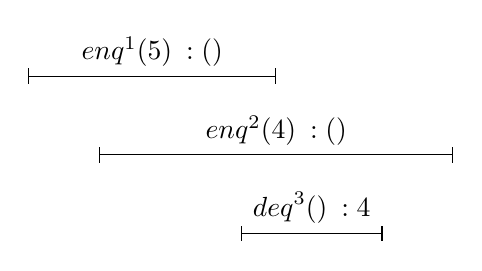
\begin{tikzpicture}[xscale = 0.9]
\draw[|-|] (0,0) -- node[above] {$\sm{enq}^1(5)\::()$} (3.5,0);
\draw (2.5,0) \X;
\draw[|-|] (1,-1) -- node[above] {$\sm{enq}^2(4)\::()$} (6,-1);
\draw (2,-1) \X;
\draw[|-|] (3,-2) -- node[above] {$\sm{deq}^3()\::4$} (5,-2);
\draw (4,-2) \X;
\end{tikzpicture}
\end{center}
\caption{Timeline representing the linearisation example.  Time runs from left
  to right; each horizontal line represents an operation execution, with the
  left-hand end representing the $\call$ event, and the right-hand end
  representing the $\return$ event.}
\label{fig:lin-timeline}
\scalaMid
\end{figure}

%%%%%

Linearisation is specified with respect to a specification object~$Spec$,
with the same operations (and signatures) as the concurrent object in
question. 
A history of the specification object is a sequence of events of
the form:
%
\begin{itemize}
\item $op^i(x)\::y$ representing an execution of operation~$op$ with
  parameter~$x$, returning result~$y$; again $i$~is an execution identity,
  which must appear at most once in the history.
\end{itemize}
%
A history is \emph{legal} if it is consistent with the definition of~$Spec$,
i.e.~for each execution, the precondition is satisfied, and the return value
is as for the definition of the operation in~$Spec$.  We assume that the
specification object is deterministic: after a particular history, there is a
unique value that can be returned by each execution.

For example, consider the history
\begin{eqnarray*}
h_s & = & \seq{\sm{enq}^2(4)\::(),\; \sm{enq}^1(5)\::(),\; \sm{deq}^3()\::4}.
\end{eqnarray*}
%
This is a legal history for a specification object that represents a queue.
This history is illustrated by the ``$\cross$''s in
Figure~\ref{fig:lin-timeline}.

Let $h$ be a complete concurrent history, and let $h_s$ be a legal history of
the specification object.  We say that $h$ and~$h_s$ \emph{correspond} if they
contain the same executions, i.e., for each $\call.op^i(x)$ and
$\return.op^i\::y$ in $h$,\, $h_s$ contains $op^i(x)\::y$, and vice versa.  We
say that $h_s$ is a \emph{linearisation} of~$h$ if there is some way of
interleaving the two histories (i.e.~creating a history containing the events
of~$h$ and~$h_s$, preserving the order of events) such that each $op^i(x)\::y$
occurs between $\call.op^i(x)$ and $\return.op^i\::y$.  Informally, this
indicates that the executions of~$h$ appeared to take place in the order
described by~$h_s$, and that this order is legal according to the
specification object.
%% We say that $h$ is \emph{linearisable} in this case.

Continuing the running example, $h_s$ is a linearisation of~$h$, as evidenced
by the interleaving
\[
\seq{\begin{align}
  \call.\sm{enq}^1(5),\; \call.\sm{enq}^2(4),\; 
  \sm{enq}^2(4)\::(),\; \sm{enq}^1(5)\::(),\;   \call.\sm{deq}^3(), \\
  \return.\sm{enq}^1\::(),\; \sm{deq}^3\::4,\; 
  \return.\sm{deq}^3\::4,\; \return.\sm{enq}^2\::() },
  \end{align}
\]
as illustrated in  Figure~\ref{fig:lin-timeline}.

A concurrent history might not be complete, i.e.~it might have some pending
executions that have been called but have not returned.  An \emph{extension}
of a history~$h$ is formed by adding zero or more $\return$ events
corresponding to pending executions.  We write $complete(h)$ for the
subsequence of~$h$ formed by removing all $\call$ events corresponding to
pending executions.
%
We say that a (not necessarily complete) concurrent history~$h$ is
\emph{linearisable} if there is an extension~$h'$ of~$h$ such that
$complete(h')$ is linearisable.  We say that a concurrent object is
linearisable if all of its histories are linearisable. 

%%%%%%%%%%%%%%%%%%%%%%%%%%%%%%%%%%%%%%%%%%%%%%%%%%%%%%%%%%%%

\subsection{Synchronisation linearisation}
\label{sec:sync-lin}

We now adapt the definition of linearisation to synchronisations.  For the
moment, we consider only binary synchronisations.  We
consider a concurrent history of the synchronisation object~$Sync$.  The
history contains $\call$ and $\return$ events, as in the previous subsection;
in the case of binary synchronisations, the events correspond to the
operations~$\op_1$ and~$\op_2$.

For example, the following is a complete history of the synchronous channel
from earlier, and is illustrated in Figure~\ref{fig:sync-timeline}:
\begin{eqnarray*}
h & = & 
\seq{\begin{align}
  \call.\sm{send}^1(8),\; \call.\sm{send}^2(8),\; \call.\sm{receive}^3(()),\;
  \return.\sm{receive}^3\::8,\; \\
  \call.\sm{receive}^4(()),\; \return.\sm{send}^1\::(),\;
  \call.\sm{send}^5(9),\; \return.\sm{receive}^4\::9,\; \\
  \call.\sm{receive}^6(()),\; \return.\sm{send}^2\::(), \;
  \return.\sm{send}^5\::(),\; \return.\sm{receive}^6\::8 } .
  \end{align}
\end{eqnarray*}

%%%%%

\begin{figure}
\unScalaMid
\begin{center}
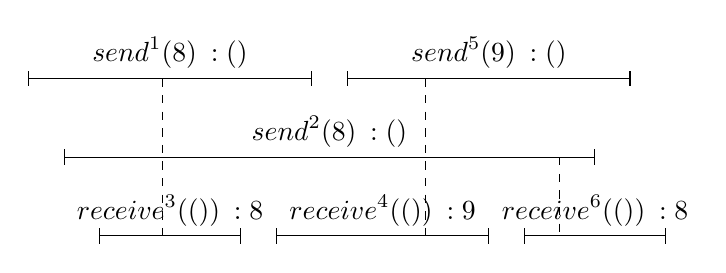
\begin{tikzpicture}[xscale = 0.9]
\draw[|-|] (0,0) -- node[above] {$\sm{send}^1(8)\::()$} (4,0);
\draw[|-|] (4.5,0) -- node[above] {$\sm{send}^5(9)\::()$} (8.5,0);
\draw[|-|] (0.5,-1) -- node[above] {$\sm{send}^2(8)\::()$} (8,-1);
\draw[|-|] (1,-2) -- node[above] {$\sm{receive}^3(())\::8$} (3,-2);
\draw[|-|] (3.5,-2) -- node[above] {$\sm{receive}^4(())\::9$} (6.5,-2);
\draw[|-|] (7,-2) -- node[above] {$\sm{receive}^6(())\::8$} (9,-2);
\draw (1.9,0) \X; \draw (1.9,-2) \X; 
\draw[dashed] (1.9,0) -- (1.9,-2); % sync 1 and 3
\draw (5.6,0) \X; \draw (5.6,-2) \X; 
\draw[dashed] (5.6,0) -- (5.6,-2); % sync 4 and 5
\draw (7.5,-1) \X; \draw (7.5,-2) \X; 
\draw[dashed] (7.5,-1) -- (7.5,-2); % sync 2 and 6 
\end{tikzpicture}
\end{center}
\caption{Timeline representing the synchronisation example.}
\label{fig:sync-timeline}
\scalaMid
\end{figure}


A history of a synchronisation specification object $Spec$ is a sequence of
events of the form $\sync^{i_1, i_2}(x_1, x_2)\:: (y_1, y_2)$, representing an
execution of |sync| with parameters $(x_1, x_2)$ and result $(y_1,y_2)$.  The
event's  identity is~$(i_1,i_2)$: each of~$i_1$ and~$i_2$ must
appear at most once in the history.  Informally, an event $\sync^{i_1,
  i_2}(x_1, x_2)\:: (y_1, y_2)$ corresponds to a synchronisation between
executions $\op_1^{i_1}(x_1)\::y_1$ and $\op_2^{i_2}(x_2)\::y_2$ in a history
of the corresponding synchronisation object.

A history is \emph{legal} if is consistent with the definition of the
specification object.
%
For example, the following is a legal history of |SyncChanSpec|.
\begin{eqnarray*}
h_s & = & 
\seq{
 \sm{sync}^{1,3}(8,()) \:: ((), 8), \;
 \sm{sync}^{5,4}(9,()) \:: ((), 9), \;
 \sm{sync}^{2,6}(8,()) \:: ((), 8) } .
\end{eqnarray*}
The history is illustrated by the ``$\cross$''s in
Figure~\ref{fig:sync-timeline}: each event corresponds to the synchronisation
of two operations, so is depicted by two ``$\cross$''s on the corresponding
operations, linked by a dashed vertical line.  This particular synchronisation
specification object is stateless, so in fact any permutation of this history
would also be legal (but not all such permutations will be compatible with the
history of the synchronisation object); but the same will not be true in
general of a specification object with state.
%
\begin{definition}
Let $h$ be a complete history of the synchronisation object~$Sync$.  We say
that a legal history~$h_s$ of~$Spec$ \emph{corresponds} to~$h$ if their
identities agree; more precisely:
%
\begin{itemize}
\item For each |sync| event with identity~$(i_1,i_2)$ in~$h_s$,\, $h$ contains
  an execution of~$\op_1$ with identity~$i_1$ and an execution of~$\op_2$ with
  identity~$i_2$;

\item For each execution of~$\op_1$ with identity~$i_1$ in~$h$,\, $h_s$
  contains a |sync| event with identity~$(i_1,i_2)$ for some~$i_2$;

\item For each execution of~$\op_2$ with identity~$i_2$ in~$h$,\, $h_s$
  contains a |sync| event with identity~$(i_1,i_2)$ for some~$i_1$.
\end{itemize}
\end{definition}

\begin{definition}
Given a complete history $h$ of~$Sync$ and a corresponding legal history $h_s$
of~$Spec$, we say that $h_s$ is a \emph{synchronisation linearisation} of~$h$
if there is some way of interleaving $h$ and~$h_s$ such that each event
$\sync^{i_1, i_2}(x_1, x_2)\:: (y_1, y_2)$ occurs between
$\call.\op_1^{i_1}(x_1)$ and $\return.\op_1^{i_1}\::y_1$, and between
$\call.\op_2^{i_2}(x_2)$ and $\return.\op_2^{i_2}\::y_2$.
\end{definition}
%
% We say that $h$ is \emph{synchronisation linearisable} in this case.
In~the running example, $h_s$ is a synchronisation linearisation of~$h$,
as shown by the interleaving in Figure~\ref{fig:sync-timeline}.

\begin{definition}
Given a (not necessarily complete) concurrent history~$h$ and a corresponding
legal history~$h_s$ of $Spec$, we say that $h_s$ is a \emph{synchronisation
  linearisation} of~$h$ if there is an extension~$h'$ of~$h$ such that $h_s$
is a synchronisation linearisation of $complete(h')$.
%
We say that $h$ is synchronisation-linearisable in this case.  We say that a
synchronisation object is synchronisation-linearisable if all of its histories
are synchronisation-linearisable.
\end{definition}

%  \framebox{Is the definition compositional?}  I think so.
